\chapter{Pre-trained Language Model for Web-scale Retrieval in Baidu Search}

\textbf{Reference:}~\url{https://arxiv.org/abs/2106.03373}

\textbf{Keywords:} transformers, retrieval \\

Трансформеры находят все большую популярность в задачах информационного поиска.
Ранее мы уже обсуждали\footnote{\url{https://vk.com/papersreaders?w=wall-154085965_402}}, то как Microsoft использует BERT для отбора кандидатов при ранжировании поисковой выдачи, сейчас речь пойдем о том как Baidu использует ERNIE для решения этой задачи.

Работа интересна еще и потому что авторы уделяют большое внимание вопросу того как подобное решение заводить в высоконагруженном продакеше.

\section*{Какую задачу решают авторы?}

Для эффективного поиска документов в интернете одного только полнотекстового поиска (\textit{text matching}) недостаточно. Эта проблема особенно остро стоит для редких поисковых запросов. 
Для решения данной проблемы все чаще используют смесь из полнотекстового и семантического поиска (\textit{semantic matching}).

В отличии от полнотекстового поиска семантический позволяет оценивать смысловую схожесть текстов даже если в них нет общих слов.
Для моделирования семантической близости текстов чаще всего используют подходы на основе нейросетей, например таких как DSSM или BERT. \\

BERT позволяет добиться sota результатов на большом количестве задач, но в исходном виде его нельзя использовать для оценики семантической близости между запросом и документом из-за особенностей архитектуры.
Напомним, что BERT для оценки схожести текстов принимает на вход оба текста сконкатенированных SEP токеном. 
В тоже время, для эффективного отбора документов кандидатов при поиске нам бы хотелось иметь возможность получить векторное представление для запроса и быстро найти множество ближайших документов в терминах близости между векторами. 
То есть, нам в онлайне нужно иметь доступ к заранее подготовленным векторам для корпуса документов.
BERT в своем исходном виде не позволяет получить отдельные векторные представления для документов и запросов. \\

Один из способов решения данной проблемы был предложен исследователями из Microsoft, которые сначала обучили BERT на поисковых логах, а затем выполнили \textit{knowledge distillation} (KD) из данной модели в two-tower BERT модель~\cite{lu2020twinbert}, которая может быть эффективно использована в интернет-поиске. \\

В рамках данной работы авторы предлагают много этапную схему \textit{fine-tuning}'а предобученной модели без использования KD, которая позволяет построить two-tower модель.

\section*{Как решают?}

Рассмотрим сначала детальнее то из каких этапов состоит пайплайн обучения модели, а затем посмотрим на то как предложенная модель используется в онлайне для отбора документов-кандидатов и при ранжировании итоговой поисковой выдачи.

\subsection*{Обучение}

Процесс обучения состоит из нескольких этапов (см. Рисунок~\ref{fig:baidu_training_pipeline}).

\begin{figure}[ht]
  \centering
  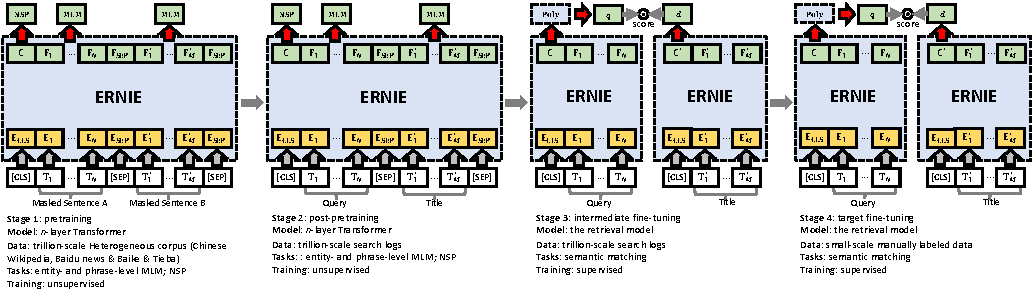
\includegraphics[width=1.1\linewidth]{figures/baidu-training-pipeline.pdf}
  \caption{\footnotesize{Training Paradigm of ERNIE-based Retrieval Model}}
  \label{fig:baidu_training_pipeline}
\end{figure}

\paragraph{Stage 1: pretraining} На первом шаге выполняется обучение модели ERNIE на большом корпусе текстов.
Модель обучают классическим для трансформеров способом - решают задачи \textit{Masked Language Modeling (MLM)} и \textit{Next Sentence Prediction (NSP)}
Фактически тут можно воспользоваться уже предобученной моделью, которых существует большое множество.

\paragraph{Stage 2: post-pretraining} В рамках данного этапа в модель превносится знание о предметной област - модель дообучается на поисковых логах. 
При этом так же как и раньше решаются задачи MLM и NSP.

\paragraph{Stage 3: intermediate fine-tuning} На данном шаге обученный ранее энкодер используется для получения векторных представлений запроса и документа.
Модель обучают решать задачу \textit{semantic matching}, используя поисковые логи.

Важно отметить, что в отличии, например, от DSSM или TwinBERT, в рамках данной работы для получения векторов запроса и документа используется \textit{один и тот же энкодер}.

Так же на данном этапе обучается новый фрагмент модели \textit{Poly-attention}, но для конспекта это не так важно.

После этого шага модель уже намного больше знает о задаче поиска.

\paragraph{Stage 4: target fine-tuning} Остается только дообучить модель на более качественном датасете, размеченном экспертами, для того чтобы сделать модель еще лучше.

\subsection*{Deployment}

Рассмотрим в кратце несколько практических приемов, которые позволили вывести данное решение в продакшн окружение.

\paragraph{Compression} Как правило, векторные представление полученные с помощью трансформеров имеют достаточно большую размерность (в данной работе - $768$).
Размерность полученных векторов в данном случае имеет очень большое значение, так как напрямую влияет на то сколько места потребуется для хранения всех векторов документов. \\

Для того чтобы уменьшить требуемый объем памяти, авторы предлагают \textit{сжать} вектора уменьшив их размерность.
Для этого во время обучения модели вместе с ней обучается еще и дополнительный \textit{fully-connected} слой, который переводит вектора из исходного пространства в новое размерностью $256$, с сохранением свойств исходного пространства. \\

Для того чтобы тратить на хранение векторов еще меньше памяти, авторы дополнительно выполняют \textit{Quantization}.

\paragraph{Production} На Рисунке~\ref{fig:baidu_system} представлена общая схема использования ERNIE в продакшн системе поиска Baidu.

\begin{figure}[ht]
  \centering
  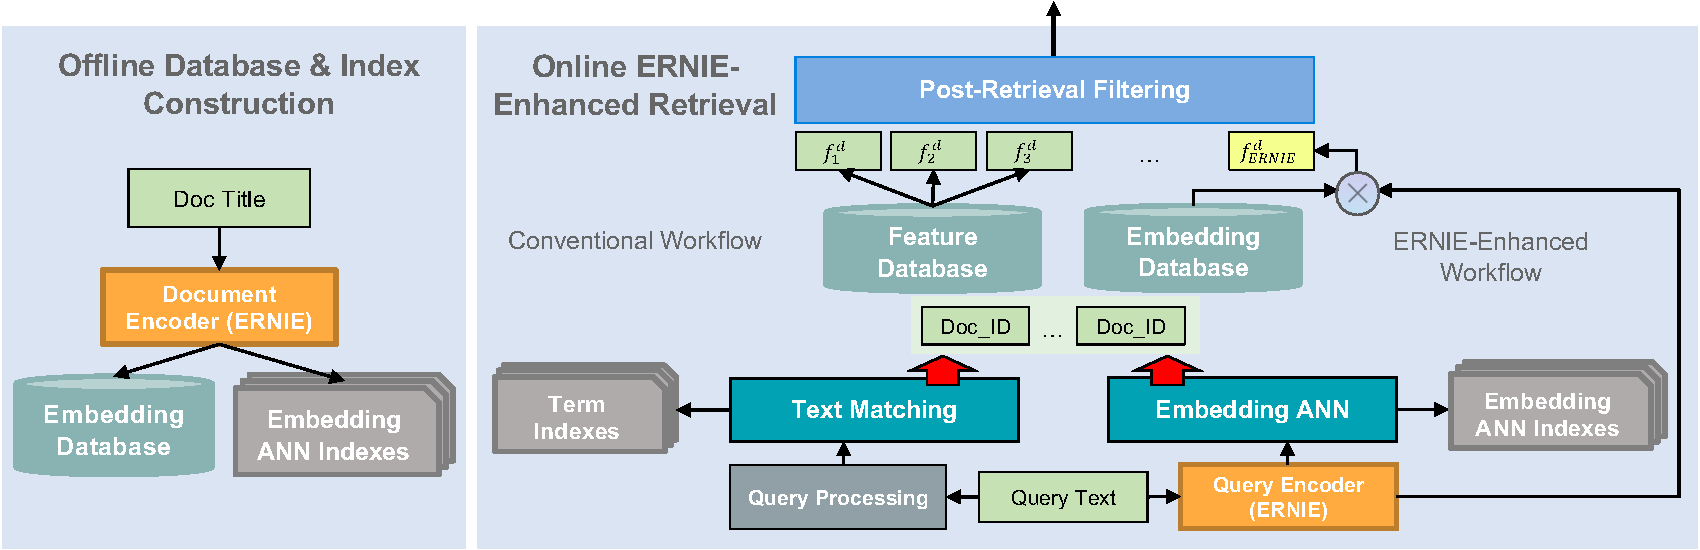
\includegraphics[width=1.0\linewidth]{figures/baidu-system.pdf}
  \caption{\footnotesize{The overall workflow of the ERNIE-enhanced retrieval system}}
  \label{fig:baidu_system}
\end{figure}

Авторы не заменяют целиком полнотекстовый поиск, а используют ERNIE как дополнение к нему для получения дополнительного набора документов-кандидатов при ранжировании.

Кроме того, меру семантической схожести между запросом и документом считают для всех извлеченных документов-кандидатов.
Вычисленные значения используются далее моделью, которая ранжирует документы для построения финальной выдачи. 

Авторы отмечают, что даже одно только добавление признака на основе ERNIE для модели ранжирования позволяет существенно улучшить качество системы, а использование ERNIE еще и для извлечения кандидатов позволят добиться еще лучших результатов.

\paragraph{Experiments} Авторы проводят AB тесты по сравнению нового решения с их текущей продакшн системой, в рамках которых показывают, что новое решение намного лучше (особенно на редких запросах).

\section*{Мое мнение}

Статья мне кажется довольно интересной еще и потому что в ней, в отличии от большинства современных работ, довольно большое внимание уделено продакшн составляющей и онлайн экспериментам.
Поэтому статья позволяет получить некоторое, пусть даже и поверхностное, представление о том как работают современные поисковые системы даже тем, кто почти ничего про это не знает.